\begin{figure}[!ht]
	\centering
	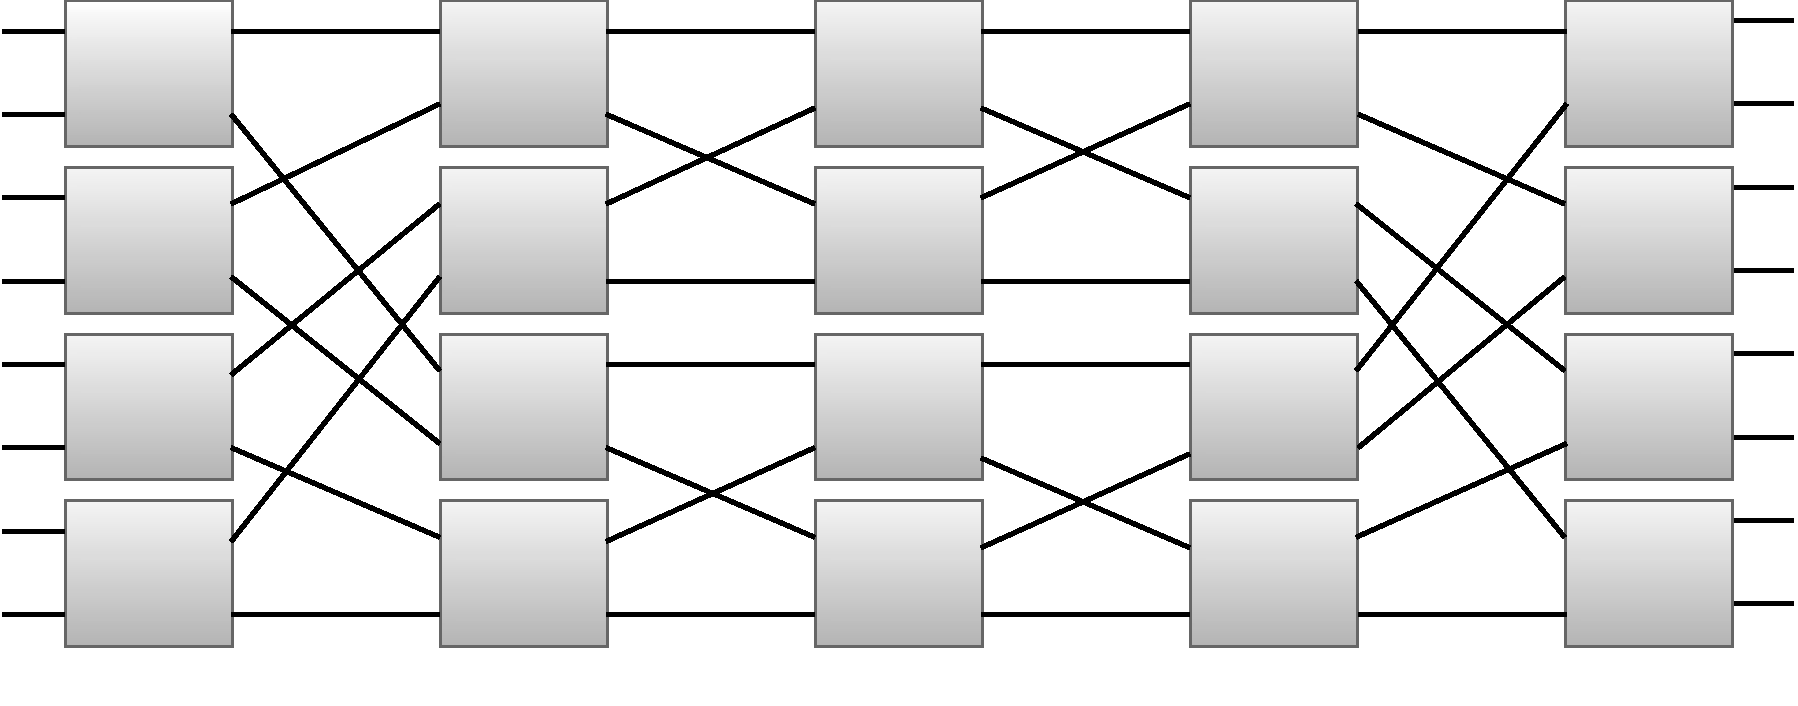
\includegraphics[width=0.7\linewidth]{benes_network.pdf}
	\caption{The basic structure of a Beneš network}
	\label{fig:benes}
\end{figure}

The Beneš network is an extension of the Banyan network.
It solves the problem that a Banyan network is not able to produce all possible permutations by mirroring the Banyan network and connecting the two.
An example for a Beneš network with 8 inputs is given in Figure \ref{fig:benes}.

The two halves of the network are different in the routing procedure employed.
For the output half, the destination of a data packet defines the exact setting of every switch on its path, because there always is only one possible choice.
The input half is responsible for conflict avoidance, which has a significantly higher complexity due to the fact that it depends on all inputs of one column of the network.

\begin{figure}[!ht]
	\centering
	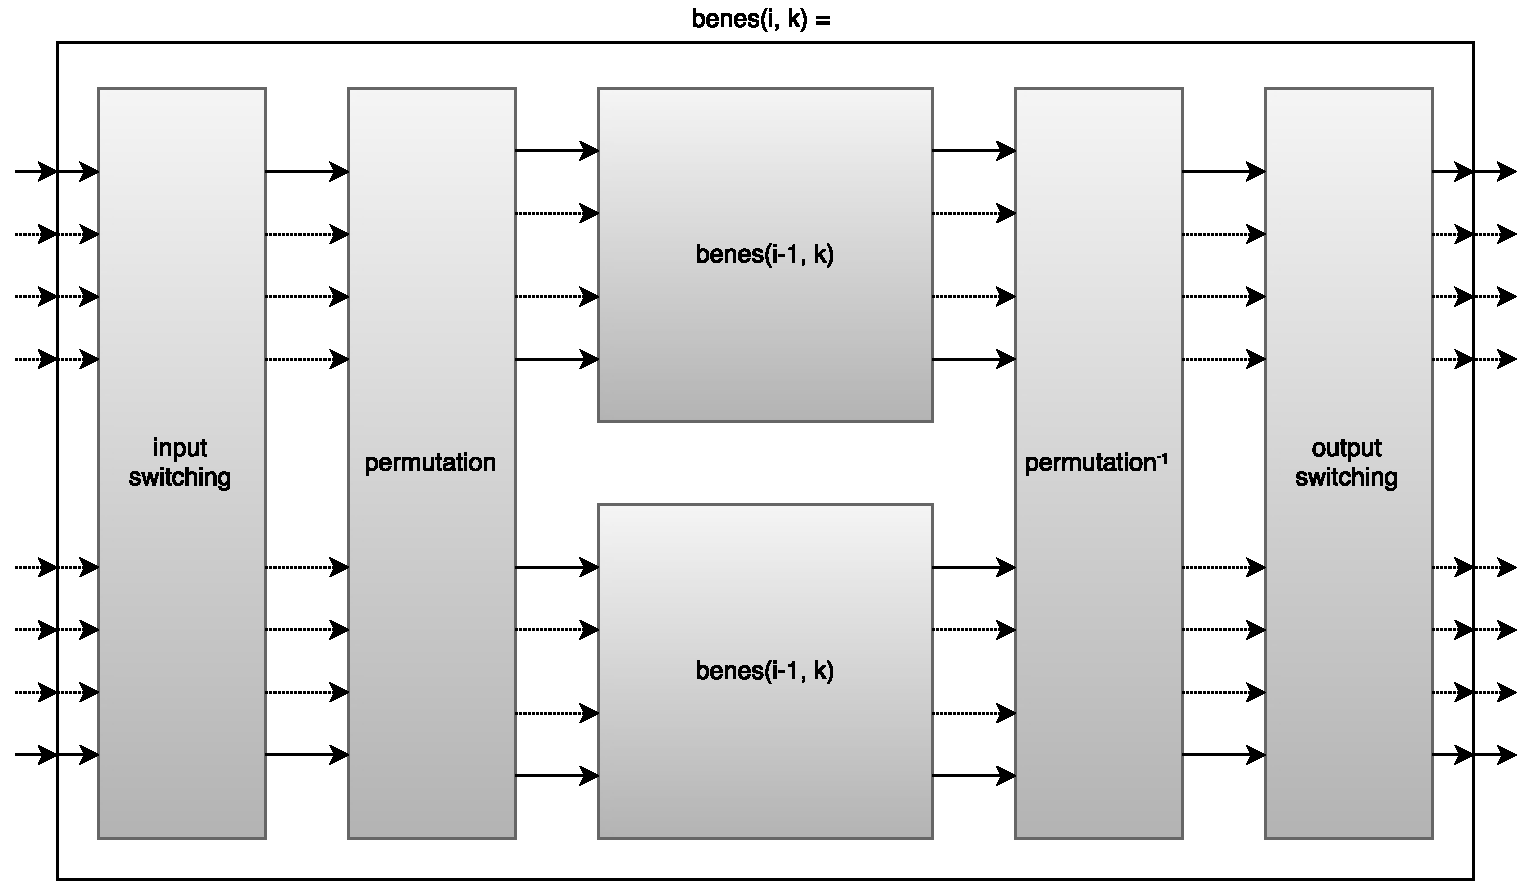
\includegraphics[width=0.7\linewidth]{benes_recursion.pdf}
	\caption{Recursive definition of a Beneš network}
	\label{fig:benes_recursion}
\end{figure}

For implementation, the recursive structure given in Figure \ref{fig:benes_recursion} was used.
A network with $2^n$ inputs is defined as $benes(n, n)$, where the first parameter gives the size of the specific network defined, and the second is used during recursion to remember the size of the whole network.

For this structure, the routing decision of the output switches is based on just bit $k - 1$, where a $0$ requires the packet to go up and $1$ to go down.

\begin{figure}[!ht]
	\centering
	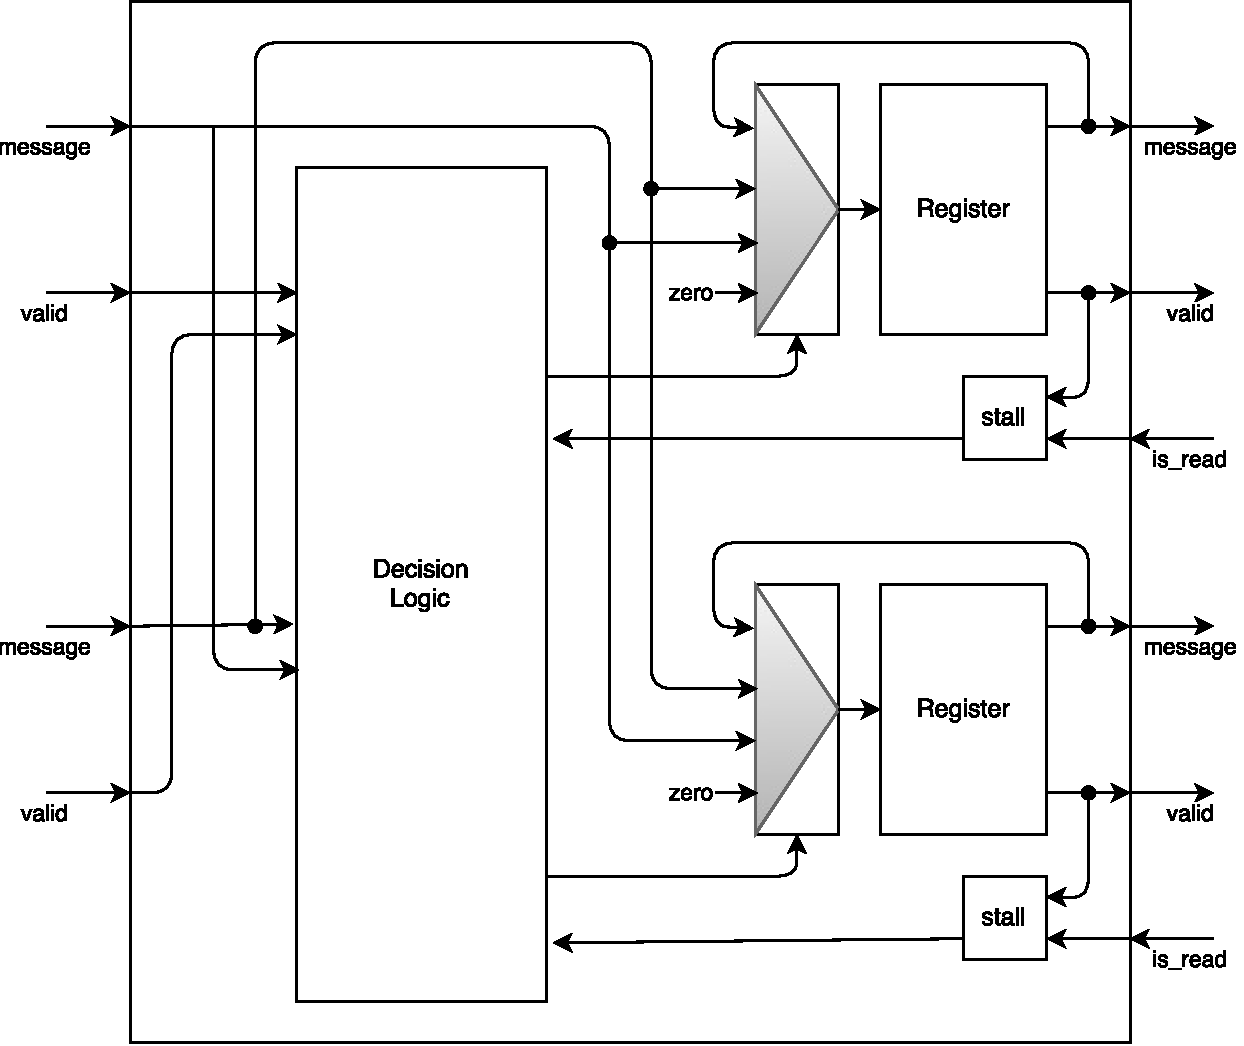
\includegraphics[width=0.7\linewidth]{banyan_stall_switch.pdf}
	\caption{Structure of stalling banyan network switches}
	\label{fig:banyan_stall_switch}
\end{figure}

Together with the necessary registers for a pipelined network, the structure of those output switches is given in Figure \ref{fig:banyan_stall_switch}.
The second half of the Beneš network, the stalling Banyan, is built using only these switches, and requires only a minimal amount of logic (see Section \ref{sec:benes_resource_utilisation}) for a functionally complete DTN.

\begin{figure}[!ht]
	\centering
	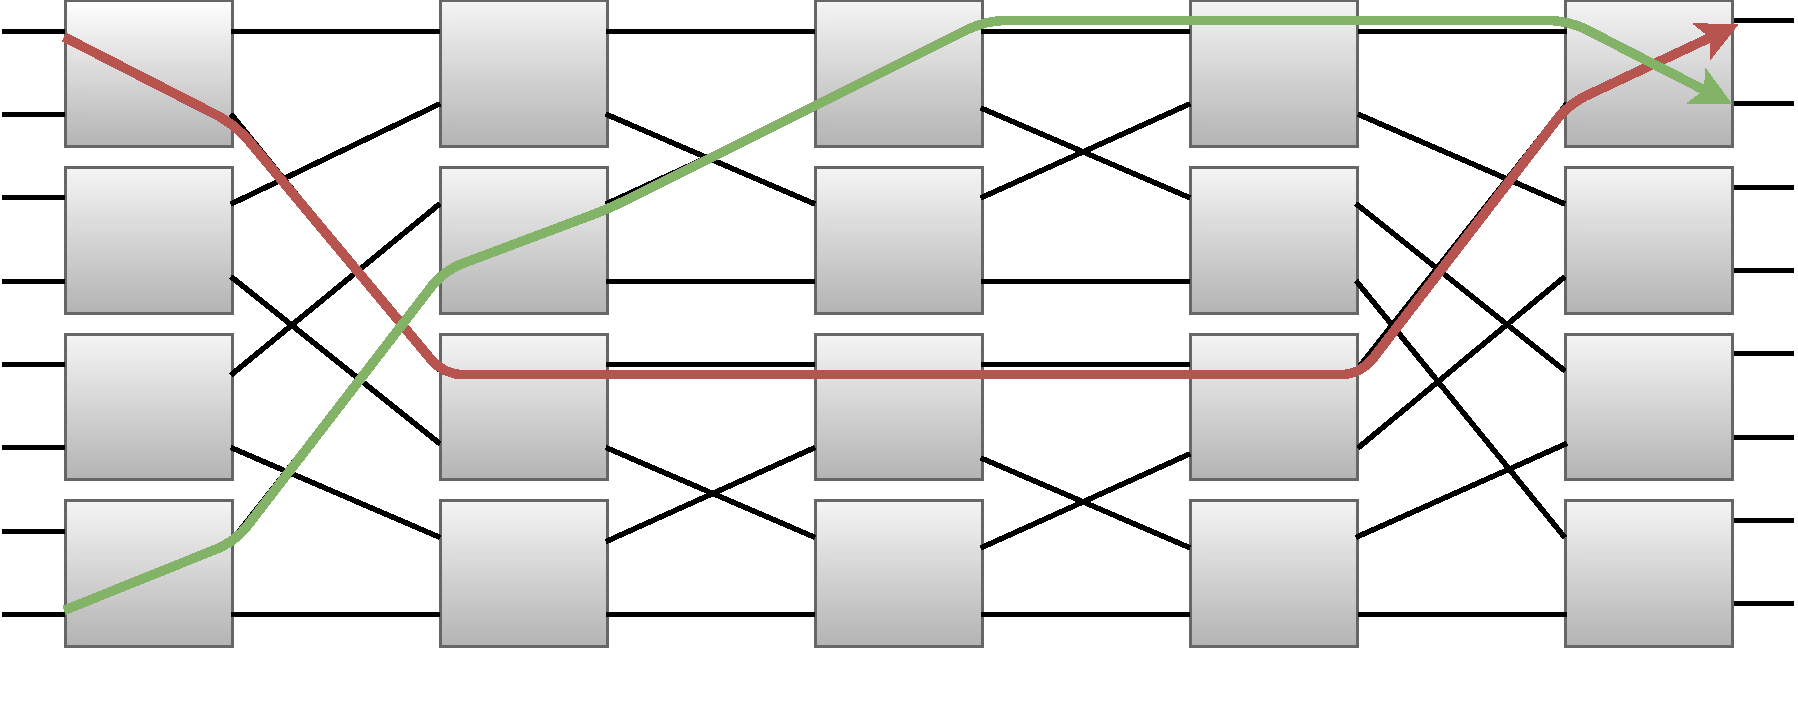
\includegraphics[width=0.7\linewidth]{benes_companions.pdf}
	\caption{Paths of two outermost-layer companions}
	\label{fig:benes_companions}
\end{figure}

Causing more complexity, the routing decisions for the input switches of the Beneš network depend on all inputs of the network.
This is due to the fact that each pair of messages comes to an output switch has to arrive from two different subnetworks.
An example illustrating this is shown in Figure \ref{fig:benes_companions}.
Each destination address has a "companion", that is routed to the same output switch.

\begin{figure}[!ht]
	\centering
	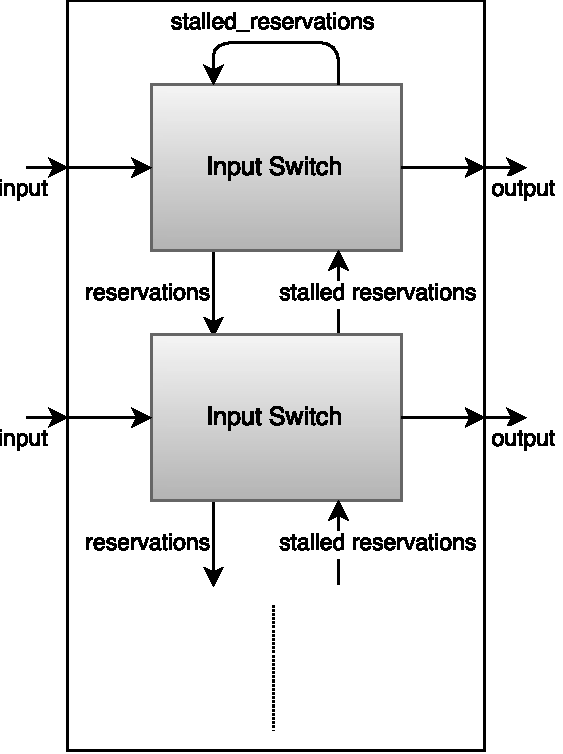
\includegraphics[width=0.3\linewidth]{benes_input_column.pdf}
	\caption{Structur of Beneš network input switch column}
	\label{fig:benes_switchcolumn_in}
\end{figure}

\begin{figure}[!ht]
	\centering
	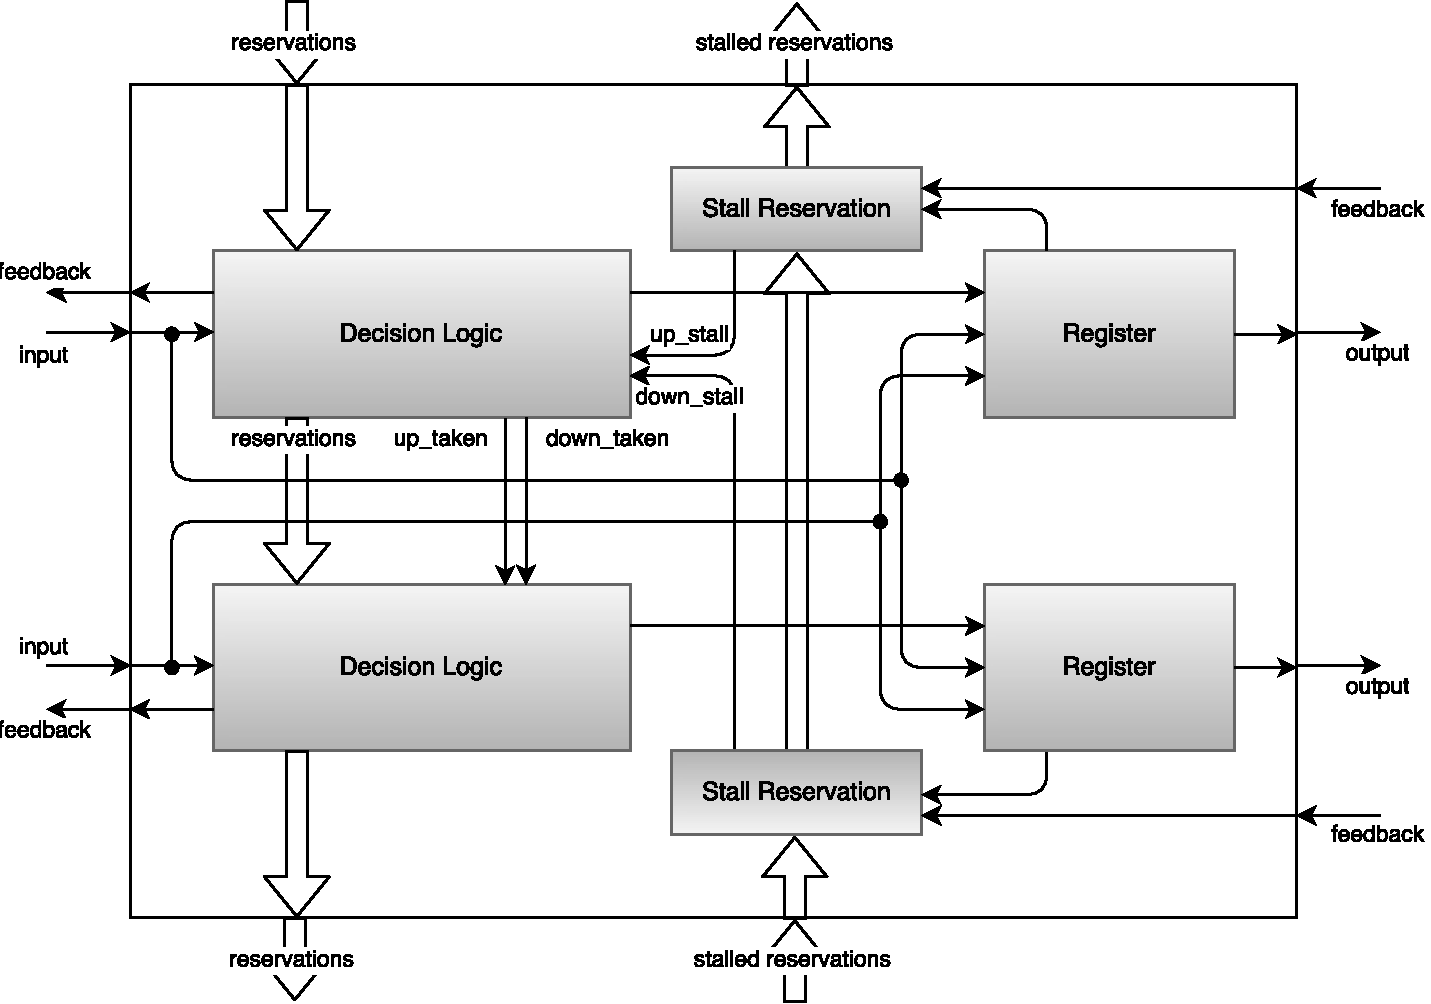
\includegraphics[width=0.8\linewidth]{benes_input_switch.pdf}
	\caption{Functional overview of Beneš input switch}
	\label{fig:benes_switch_in}
\end{figure}

To handle these dependencies properly, the input switch column of the recursive Beneš network uses reservation signals, where specific destinations are reserved by the switches sending packets to them so they are sent only once.
This is shown in Figure \ref{fig:benes_switchcolumn_in}, along with the lines for reservations from stalled packets, which need to have the highest priority because they can not be held back in the current architecture.
A detailed overview of an input switch is given in Figure \ref{fig:benes_switch_in}.

As a more simple solution, a lookup table for the first stage of a $32\times32$ Beneš network would require around $2.92\times10^{48}$ bytes.


\FloatBarrier
\subsubsection{Message Ordering}

		For each packet from source $s$ and destination $d$ and for the program order of move instructions $m_n(s_n, d_n) \prec m_{n+1}(s_{n+1}, d_{n+1})$, and delivery order of network $m_n \lhd m_k$, the following constraint has to hold:
	\begin{align*}
		& (m_n(s_n, d_n) \prec m_k(s_k, d_k)) \wedge (s_n = s_k \wedge d_n = d_k) \\
		& \Rightarrow (m_n(s_n, d_n) \lhd m_k(s_k, d_k))
	\end{align*}

	This is necessary since the input buffers cannot distinguish between different packets that have equal sources and destinations.
	
	With the recursive structure of the Beneš network and possible stalling at each input step, this constraint can not be guaranteed and is a case for which the network might work incorrectly.
	This does not apply to the Banyan part of the network, since relevant message pairs take the same path and do not overtake each other.
	
\subsubsection{Resource Utilisation of the Beneš Network}
	\label{sec:benes_resource_utilisation}
	\begin{table}[!ht]
		
		\begin{center}
			\begin{tabular}{l | c | c }
				\textbf{Site Type}  & \textbf{Benes(\%)}&\textbf{Stalling Banyan(\%)} \\
				\hline \hline
				Slice LUTs          & 51.23             & 13.86 \\
				\quad LUT as Logic  & 51.23             & 13.86 \\
				\quad LUT as Memory & 0.00              & 0.00  \\
				Slice Registers     & 12.28             & 06.61 \\
				\quad Register as Flip Flop & 12.28     & 06.61 \\
				\quad Register as Latch     & 0.00      & 0.00  \\
				F7 Muxes                    & 1.53      & 0.00  \\
				F8 Muxes                    & 0.63      & 0.00 \\
			\end{tabular}
		\end{center}
		\caption{Resource utilization of DTN with Benes network}
		\label{fig:benes_utilisation}
	\end{table}
	
	As shown in Table \ref{fig:benes_utilisation}, the Beneš network takes significantly more logic than all other DTNs.
	This, together with the high circuit depth required, make this implementation an unsuitable candidate for the SCAD architecture data network.
	
	The stalling banyan network may be considered for applications where a small DTN is required.
